\documentclass[11pt]{article}

\usepackage{amsmath, amssymb, amsthm}
\usepackage{tikz}

\theoremstyle{plain}
\newtheorem{thm}{Theorem}[section]
\newtheorem*{thm*}{Theorem}
\newtheorem{prop}[thm]{Proposition}
\newtheorem{lem}[thm]{Lemma}
\newtheorem*{lem*}{Lemma}
\newtheorem{dfn}[thm]{Definition}
\newtheorem{cor}[thm]{Corollary}
\newtheorem{claim}[thm]{Claim}
\newtheorem{conj}[thm]{Conjecture}
\newtheorem{ques}[thm]{Question}
\newtheorem*{rem}{Remark}


\oddsidemargin  0pt
\evensidemargin 0pt
\marginparwidth 40pt
\marginparsep 10pt
\topmargin 0pt
\headsep 10pt
\textheight 8.2in
\textwidth 6.4in
\renewcommand{\baselinestretch}{1.1}

\newcommand{\codeg}{\text{codeg}}
\newcommand{\BBE}{\mathbb{E}}
\newcommand{\BFP}{\mathbf{P}}
\usepackage{amsmath}
\usepackage{amsthm}
\usepackage{amssymb}
\usepackage{mathtools}
\usepackage{hyperref}
\usepackage{url}





\usepackage{graphicx}
\usepackage{caption}
\usepackage{subcaption}

\def\eQb#1\eQe{\begin{eqnarray*}#1\end{eqnarray*}}
\def\eQnb#1\eQne{\begin{eqnarray}#1\end{eqnarray}}
\providecommand{\e}[1]{\ensuremath{\times 10^{#1}}}
\providecommand{\pb}[0]{\pagebreak}
\DeclarePairedDelimiter\ceil{\lceil}{\rceil}
\DeclarePairedDelimiter\floor{\lfloor}{\rfloor}

\newcommand{\E}{\mathrm{E}}
\newcommand{\Var}{\mathrm{Var}}
\newcommand{\Cov}{\mathrm{Cov}}

\def\Qb#1\Qe{\begin{question}#1\end{question}}
\def\Sb#1\Se{\begin{solution}#1\end{solution}}


\newtheoremstyle{quest}{\topsep}{\topsep}{}{}{\bfseries}{}{ }{\thmname{#1}\thmnote{ #3}.}
\theoremstyle{quest}
\newtheorem*{definition}{Definition}
\newtheorem*{theorem}{Theorem}
\newtheorem*{lemma}{Lemma}
\newtheorem*{question}{Question}
\newtheorem*{preposition}{Preposition}
\newtheorem*{exercise}{Exercise}
\newtheorem*{challengeproblem}{Challenge Problem}
\newtheorem*{solution}{Solution}
\newtheorem*{remark}{Remark}
\usepackage{verbatimbox}
\usepackage{listings}
\usepackage{mathrsfs}
\date{}
\title{\vspace{-0.7cm}
PDE II: Problem Set II}

\author{
Youngduck Choi 
\thanks{Department of Mathematics, Courant Institute of Mathematical Sciences, 
yc1104@nyu.edu; If you find an error and want to share with me, 
you can reach me via email.
}}

\begin{document}

\maketitle

\begin{abstract}
This work contains solutions for the problem set II.
\end{abstract}


\begin{question}[1-1]
\hfill
\begin{figure}[h!]
  \centering
    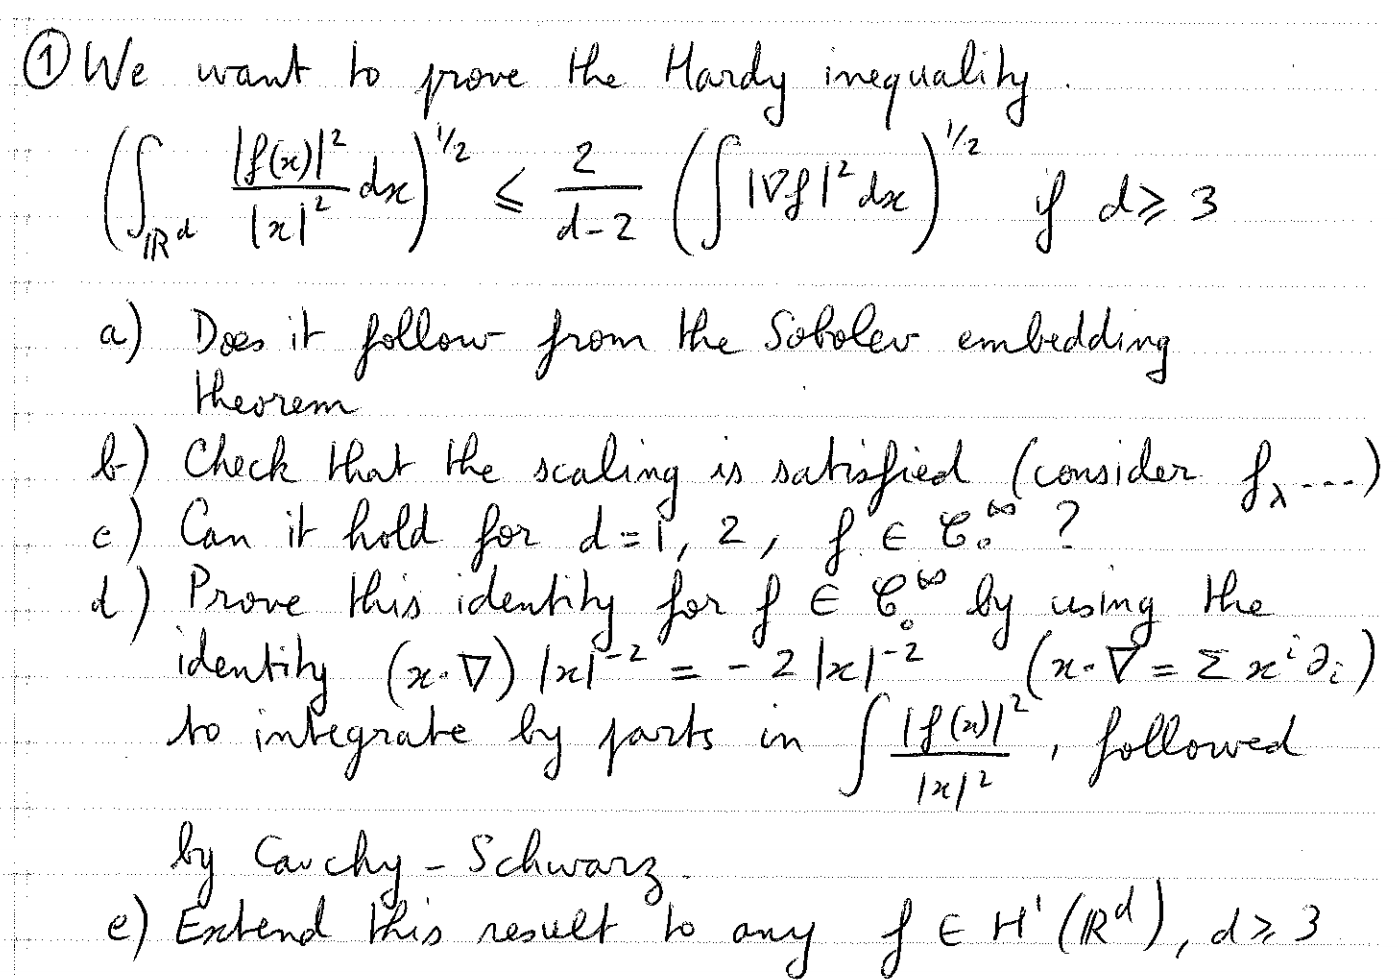
\includegraphics[width=0.7\textwidth]{pde2-s34-p1.png}
\end{figure}
\end{question}
\begin{solution} \hfill \\
\end{solution}

\newpage

\begin{question}[1-2]
\hfill
\begin{figure}[h!]
  \centering
    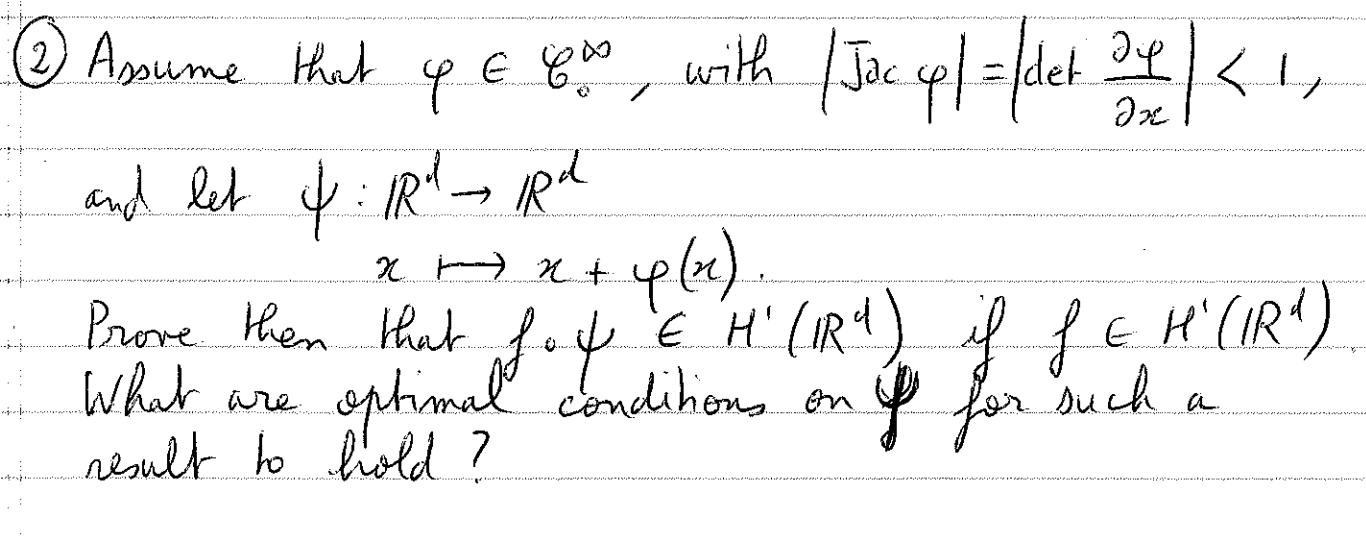
\includegraphics[width=0.7\textwidth]{pde2-s34-p2.png}
\end{figure}
\end{question}
\begin{solution} \hfill \\


\end{solution}

\newpage

\begin{question}[1-3]
\hfill
\begin{figure}[h!]
  \centering
    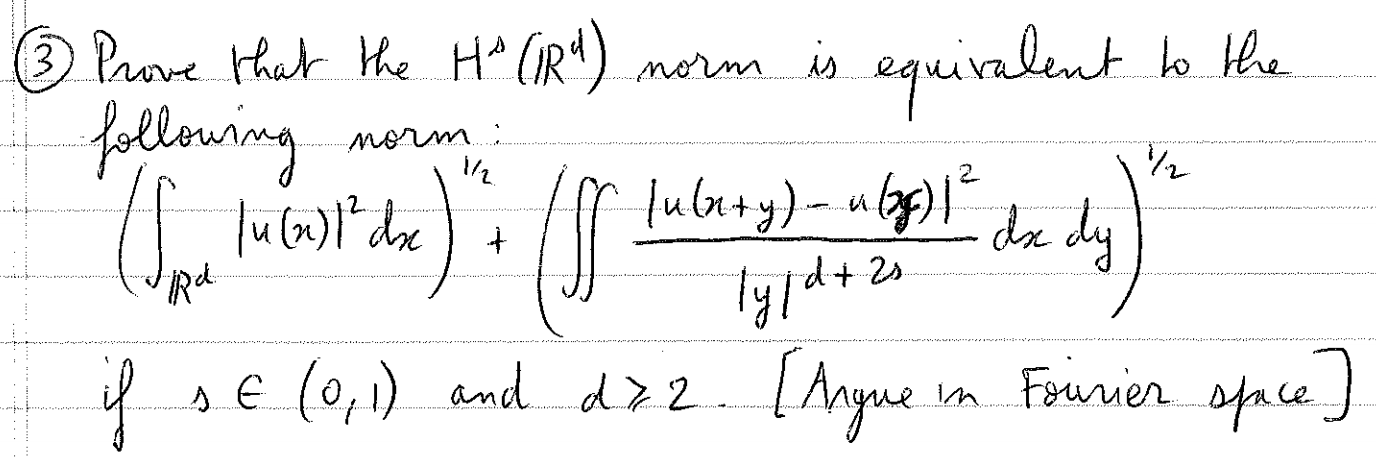
\includegraphics[width=0.7\textwidth]{pde2-s34-p3.png}
\end{figure}
\end{question}
\begin{solution} \hfill \\
\textbf{(a)}

\end{solution}

\newpage

\begin{question}[1-4]
\hfill
\begin{figure}[h!]
  \centering
    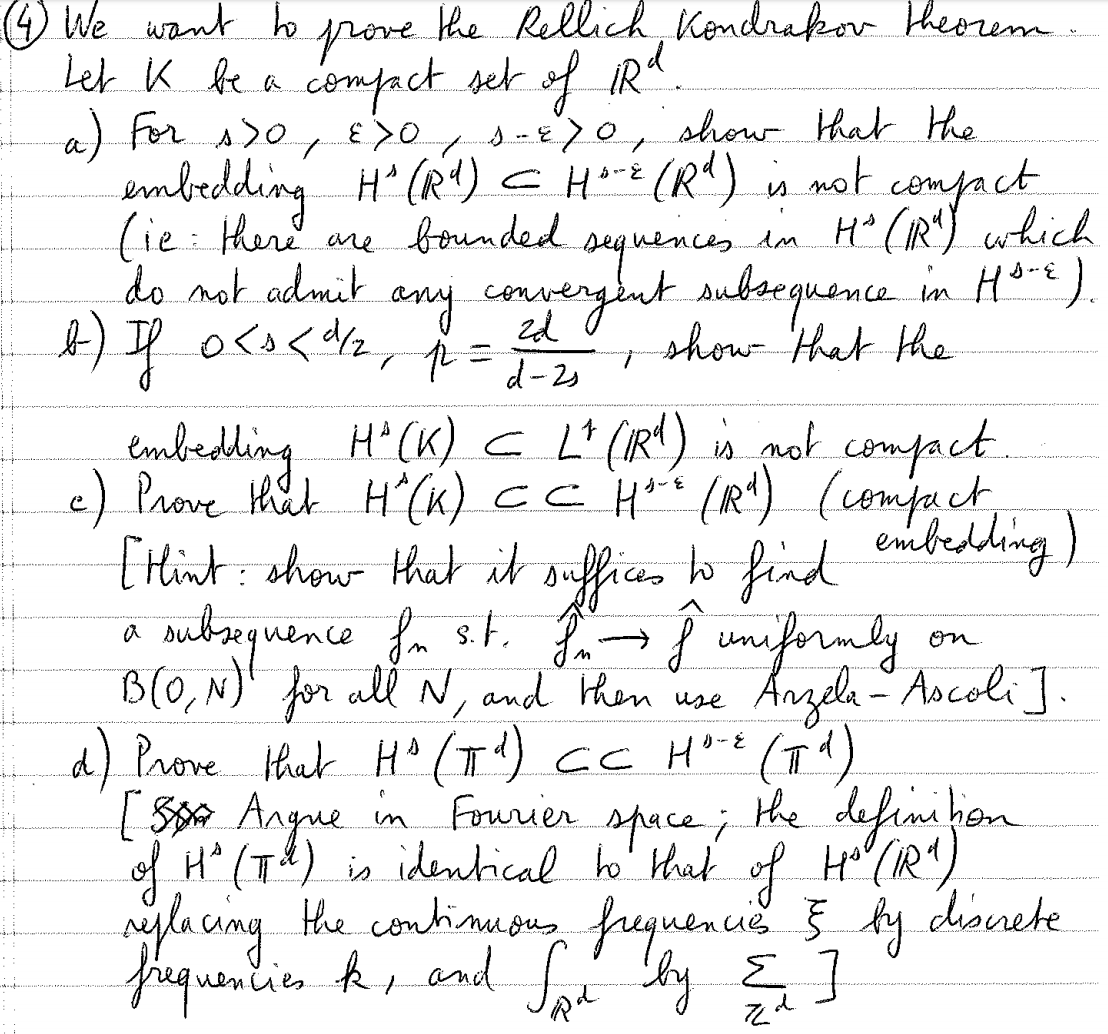
\includegraphics[width=0.7\textwidth]{pde2-s34-p4.png}
\end{figure}
\end{question}
\begin{solution} \hfill \\
\textbf{(a)}

\end{solution}
\end{document}

